% =============================================================================
% ESL FRAMEWORK - CHAPTER 2: THE K-METRIC
% =============================================================================
% Authors: Gerhard Fehr & Andrea Fehr
% FehrAdvice & Partners AG, Zürich
% Version: Extended Monograph
% =============================================================================

\documentclass[11pt,a4paper]{article}

% --- Packages ---
\usepackage[utf8]{inputenc}
\usepackage[T1]{fontenc}
\usepackage[english]{babel}
\usepackage{amsmath,amssymb,amsthm}
\usepackage{mathtools}
\usepackage{booktabs}
\usepackage{longtable}
\usepackage{hyperref}
\usepackage{geometry}
\usepackage{xcolor}
\usepackage{tcolorbox}
\usepackage{tikz}
\usepackage{pgfplots}
\usepackage{natbib}
\usepackage{enumitem}
\usepackage{fancyhdr}
\usepackage{titlesec}
\usepackage{cancel}
\pgfplotsset{compat=1.17}
\usetikzlibrary{patterns,arrows.meta,calc,positioning}

\geometry{margin=2.5cm}

% --- Colors ---
\definecolor{eslblue}{RGB}{0,82,147}
\definecolor{eslgreen}{RGB}{0,128,0}
\definecolor{eslorange}{RGB}{230,159,0}
\definecolor{eslred}{RGB}{204,51,17}
\definecolor{eslgray}{RGB}{128,128,128}
\definecolor{eslpurple}{RGB}{148,0,211}

% --- Boxes ---
\newtcolorbox{eslbox}[1][]{
  colback=eslblue!5!white,
  colframe=eslblue,
  title={ESL Assessment},
  fonttitle=\bfseries,
  #1
}

\newtcolorbox{keyinsight}[1][]{
  colback=eslgreen!5!white,
  colframe=eslgreen!80!black,
  title={Key Insight},
  fonttitle=\bfseries,
  #1
}

\newtcolorbox{warningbox}[1][]{
  colback=eslorange!5!white,
  colframe=eslorange!80!black,
  title={Methodological Note},
  fonttitle=\bfseries,
  #1
}

\newtcolorbox{proofbox}[1][]{
  colback=eslpurple!5!white,
  colframe=eslpurple!80!black,
  title={Proof},
  fonttitle=\bfseries,
  #1
}

\newtcolorbox{examplebox}[1][]{
  colback=eslgray!10!white,
  colframe=eslgray!80!black,
  title={Example},
  fonttitle=\bfseries,
  #1
}

\newtcolorbox{definitionbox}[1][]{
  colback=white,
  colframe=eslblue!80!black,
  title={Definition},
  fonttitle=\bfseries,
  #1
}

% --- Theorems ---
\newtheorem{definition}{Definition}[section]
\newtheorem{theorem}{Theorem}[section]
\newtheorem{lemma}[theorem]{Lemma}
\newtheorem{proposition}[theorem]{Proposition}
\newtheorem{corollary}[theorem]{Corollary}
\newtheorem{property}{Property}[section]
\newtheorem{axiom}{Axiom}[section]

\theoremstyle{remark}
\newtheorem{remark}{Remark}[section]

% --- Header/Footer ---
\pagestyle{fancy}
\fancyhf{}
\fancyhead[L]{\small ESL 2.3 Framework -- Extended Monograph}
\fancyhead[R]{\small Chapter 2: The K-Metric}
\fancyfoot[C]{\thepage}

% =============================================================================
% TITLE
% =============================================================================

\title{%
    \Large \textbf{Empirical Stability of Language (ESL) 2.3} \\[0.5em]
    \large A Diagnostic Quality Assurance Framework for \\
    Scientific Claim Validation \\[0.3em]
    \small \textit{``Language is a symptom, not the cause''} \\[1em]
    \LARGE \textbf{Chapter 2: The K-Metric} \\[0.3em]
    \large Mathematical Foundations, Properties, and Diagnostic Interpretation
}

\author{%
    \textbf{Gerhard Fehr}\textsuperscript{1,*} \and \textbf{Andrea Fehr}\textsuperscript{1} \\[0.5em]
    \textsuperscript{1}FehrAdvice \& Partners AG, Klausstrasse 4, 8008 Zürich, Switzerland \\[0.3em]
    \textsuperscript{*}Corresponding author: gerhard.fehr@fehradvice.com
}

\date{December 26, 2025}

\begin{document}

\maketitle

% =============================================================================
% ABSTRACT
% =============================================================================

\begin{abstract}
\noindent
This chapter presents the complete mathematical foundations of the K-metric, ESL's central formalization for measuring claim-evidence alignment. We begin with axiomatic foundations, deriving the K-metric from first principles of calibration measurement. We prove key properties including boundedness, monotonicity, symmetry conditions, and behavior under composition. The chapter introduces three K-metric variants (standard, asymmetric, and weighted) suited to different applications. We analyze the metric's geometric interpretation in B-E space, establish continuity and differentiability properties, and derive error propagation formulas for uncertainty quantification. Crucially, ESL 2.3 introduces the \textbf{diagnostic interpretation}: empirical validation ($N = 119$, $r = 0.052$ for B-value) reveals that the K-metric functions as a diagnostic indicator of underlying methodological quality, not as a causal predictor of replication success. The chapter integrates this insight with connections to M-Score and EO-Score as the true predictors.

\vspace{0.5em}
\noindent\textbf{Keywords:} K-metric, calibration measurement, diagnostic indicator, claim-evidence alignment, mathematical foundations, M-Score, EO-Score
\end{abstract}

\tableofcontents
\newpage

% =============================================================================
% 2.1 AXIOMATIC FOUNDATIONS
% =============================================================================

\section{Axiomatic Foundations}
\label{sec:axioms}

Before defining the K-metric, we establish the axiomatic requirements that any calibration metric should satisfy. These axioms constrain the space of possible metrics and motivate ESL's specific choices.

\subsection{The Calibration Measurement Problem}

We seek a function $K: [0,1] \times [0,1] \to [0,1]$ that measures the alignment between:
\begin{itemize}
    \item $B \in [0,1]$: Boldness (claim strength conveyed by linguistic markers)
    \item $E \in [0,1]$: Evidence (epistemic warrant provided by empirical support)
\end{itemize}

The function $K(B, E)$ should return high values when $B \approx E$ (good calibration) and low values when $|B - E|$ is large (poor calibration).

\subsection{Required Axioms}

\begin{axiom}[Boundedness]
\label{ax:bounded}
The calibration metric is bounded:
\begin{equation}
K: [0,1] \times [0,1] \to [0,1]
\end{equation}
This enables interpretation as a proportion or percentage of perfect calibration.
\end{axiom}

\begin{axiom}[Perfect Calibration]
\label{ax:perfect}
Perfect alignment yields maximum score:
\begin{equation}
K(B, B) = 1 \quad \forall B \in [0,1]
\end{equation}
When claim strength exactly matches evidence strength, calibration is perfect.
\end{axiom}

\begin{axiom}[Monotonicity in Deviation]
\label{ax:monotone}
$K$ decreases monotonically as $|B - E|$ increases:
\begin{equation}
|B_1 - E| < |B_2 - E| \implies K(B_1, E) > K(B_2, E)
\end{equation}
Larger claim-evidence gaps produce worse calibration scores.
\end{axiom}

\begin{axiom}[Continuity]
\label{ax:continuous}
$K$ is continuous in both arguments:
\begin{equation}
\lim_{(B', E') \to (B, E)} K(B', E') = K(B, E)
\end{equation}
Small changes in inputs produce small changes in output.
\end{axiom}

\begin{axiom}[Non-Triviality]
\label{ax:nontrivial}
$K$ is not constant:
\begin{equation}
\exists (B_1, E_1), (B_2, E_2): K(B_1, E_1) \neq K(B_2, E_2)
\end{equation}
The metric distinguishes between different calibration states.
\end{axiom}

\subsection{Optional Axioms}

The following axioms are desirable but may be relaxed for specific applications:

\begin{axiom}[Symmetry]
\label{ax:symmetry}
Overclaiming and underclaiming are penalized equally:
\begin{equation}
K(B, E) = K(E, B) \quad \forall B, E \in [0,1]
\end{equation}
\end{axiom}

\begin{axiom}[Zero at Maximum Deviation]
\label{ax:zero}
Maximum possible deviation yields minimum score:
\begin{equation}
K(0, 1) = K(1, 0) = 0
\end{equation}
\end{axiom}

\begin{keyinsight}[title={Why Symmetry May Be Undesirable}]
In scientific communication, overclaiming ($B > E$) may be more harmful than underclaiming ($B < E$):
\begin{itemize}
    \item Overclaiming propagates false confidence through the literature.
    \item Underclaiming is self-correcting (robust findings eventually gain recognition).
    \item Regulatory contexts (medicine, engineering) require conservative claims.
\end{itemize}
ESL therefore provides both symmetric and asymmetric K-metric variants.
\end{keyinsight}

% =============================================================================
% 2.2 DERIVATION OF THE K-METRIC
% =============================================================================

\section{Derivation of the K-Metric}
\label{sec:derivation}

We now derive the K-metric from the axioms, showing that it is a natural (though not unique) solution to the calibration measurement problem.

\subsection{The Deviation-Based Approach}

The simplest measure of miscalibration is the absolute deviation:
\begin{equation}
D(B, E) = |B - E|
\end{equation}

This satisfies Axioms \ref{ax:monotone} and \ref{ax:continuous}, but not Axiom \ref{ax:bounded} (since $D \in [0,1]$, not normalized to a quality score).

\subsection{Normalization Strategies}

To convert deviation to a calibration score, we need a normalization factor $N$:
\begin{equation}
K = 1 - \frac{D}{N} = 1 - \frac{|B - E|}{N}
\end{equation}

The choice of $N$ determines the metric's properties:

\begin{table}[h]
\centering
\caption{Normalization Strategies and Their Properties}
\label{tab:normalization}
\begin{tabular}{lccc}
\toprule
\textbf{Normalization} & \textbf{Formula} & \textbf{Symmetric?} & \textbf{Range} \\
\midrule
Constant ($N = 1$) & $K = 1 - |B - E|$ & Yes & $[0, 1]$ \\
Maximum ($N = \max(B, E)$) & $K = 1 - \frac{|B - E|}{\max(B, E)}$ & Yes & $[0, 1]$ \\
Boldness ($N = B$) & $K = 1 - \frac{|B - E|}{B}$ & No & $(-\infty, 1]$ \\
Evidence ($N = E$) & $K = 1 - \frac{|B - E|}{E}$ & No & $(-\infty, 1]$ \\
\bottomrule
\end{tabular}
\end{table}

\subsection{The Standard K-Metric}

\begin{definition}[Standard K-Metric]
\label{def:k-standard}
The standard K-metric uses maximum normalization:
\begin{equation}
K(B, E) = 1 - \frac{|B - E|}{\max(B, E)}
\end{equation}
with the convention that $K(0, 0) = 1$ (perfect calibration at null claim).
\end{definition}

\begin{theorem}[Standard K-Metric Satisfies Core Axioms]
\label{thm:k-axioms}
The standard K-metric satisfies Axioms \ref{ax:bounded}--\ref{ax:nontrivial} and \ref{ax:symmetry}--\ref{ax:zero}.
\end{theorem}

\begin{proofbox}
\textbf{Axiom \ref{ax:bounded} (Boundedness):}

For $B, E \in [0,1]$ with $\max(B, E) > 0$:
\begin{align}
0 \leq |B - E| \leq \max(B, E) &\implies 0 \leq \frac{|B - E|}{\max(B, E)} \leq 1 \\
&\implies 0 \leq 1 - \frac{|B - E|}{\max(B, E)} \leq 1
\end{align}

\textbf{Axiom \ref{ax:perfect} (Perfect Calibration):}
\begin{equation}
K(B, B) = 1 - \frac{|B - B|}{\max(B, B)} = 1 - \frac{0}{B} = 1 \quad \checkmark
\end{equation}

\textbf{Axiom \ref{ax:monotone} (Monotonicity):}

Let $|B_1 - E| < |B_2 - E|$ with $\max(B_1, E) = \max(B_2, E) = M$. Then:
\begin{equation}
K(B_1, E) = 1 - \frac{|B_1 - E|}{M} > 1 - \frac{|B_2 - E|}{M} = K(B_2, E) \quad \checkmark
\end{equation}

\textbf{Axiom \ref{ax:continuous} (Continuity):}

$K$ is continuous wherever $\max(B, E) > 0$ as a composition of continuous functions. At $(0, 0)$, continuity holds by definition. $\checkmark$

\textbf{Axiom \ref{ax:symmetry} (Symmetry):}
\begin{equation}
K(B, E) = 1 - \frac{|B - E|}{\max(B, E)} = 1 - \frac{|E - B|}{\max(E, B)} = K(E, B) \quad \checkmark
\end{equation}

\textbf{Axiom \ref{ax:zero} (Zero at Maximum Deviation):}
\begin{equation}
K(0, 1) = 1 - \frac{|0 - 1|}{\max(0, 1)} = 1 - \frac{1}{1} = 0 \quad \checkmark
\end{equation}
\end{proofbox}

\subsection{The Asymmetric K-Metric}

For applications prioritizing overclaiming detection:

\begin{definition}[Asymmetric K-Metric]
\label{def:k-asymmetric}
The asymmetric K-metric penalizes overclaiming more severely:
\begin{equation}
K_{\text{asym}}(B, E) =
\begin{cases}
1 - \dfrac{B - E}{B} & \text{if } B > E \text{ (overclaiming)} \\[1em]
1 - \dfrac{E - B}{E} \cdot \alpha & \text{if } B < E \text{ (underclaiming)} \\[0.5em]
1 & \text{if } B = E
\end{cases}
\end{equation}
where $\alpha \in [0, 1]$ is the underclaiming penalty weight (default: $\alpha = 0.5$).
\end{definition}

With $\alpha = 0.5$, underclaiming is penalized at half the rate of overclaiming.

\begin{examplebox}[title={Symmetric vs. Asymmetric K-Metric}]
Consider two claims:
\begin{itemize}
    \item Claim A: $B = 0.80$, $E = 0.60$ (overclaiming by 0.20)
    \item Claim B: $B = 0.60$, $E = 0.80$ (underclaiming by 0.20)
\end{itemize}

\textbf{Standard K-Metric} (symmetric):
\begin{align}
K_A &= 1 - \frac{|0.80 - 0.60|}{0.80} = 1 - 0.25 = 0.75 \\
K_B &= 1 - \frac{|0.60 - 0.80|}{0.80} = 1 - 0.25 = 0.75
\end{align}

\textbf{Asymmetric K-Metric} ($\alpha = 0.5$):
\begin{align}
K_A &= 1 - \frac{0.80 - 0.60}{0.80} = 1 - 0.25 = 0.75 \\
K_B &= 1 - \frac{0.80 - 0.60}{0.80} \cdot 0.5 = 1 - 0.125 = 0.875
\end{align}

The asymmetric metric rates underclaiming (Claim B) as better calibrated.
\end{examplebox}

% =============================================================================
% 2.3 GEOMETRIC INTERPRETATION
% =============================================================================

\section{Geometric Interpretation}
\label{sec:geometry}

The K-metric has an intuitive geometric interpretation in B-E space that clarifies its properties and suggests visualization strategies.

\subsection{The B-E Plane}

The space of all possible (claim, evidence) pairs is the unit square $[0,1] \times [0,1]$:

\begin{figure}[h]
\centering
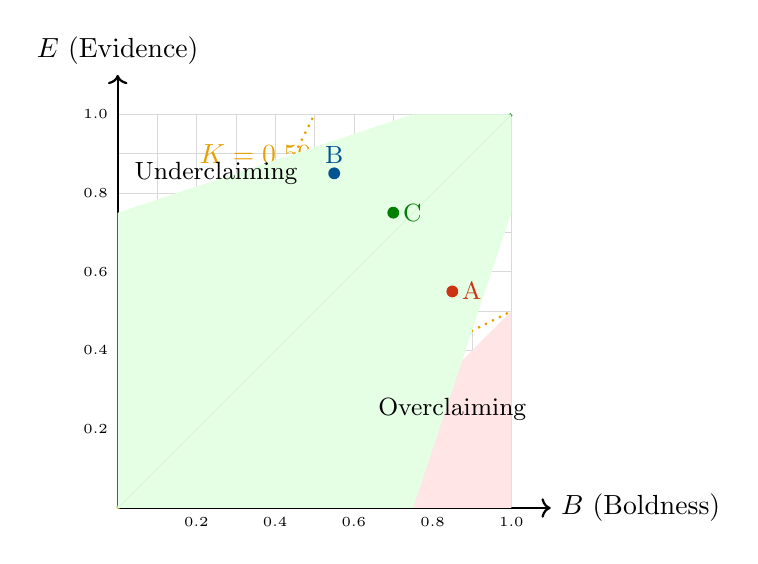
\begin{tikzpicture}[scale=5]
    % Grid
    \draw[gray!30, very thin] (0,0) grid[step=0.1] (1,1);

    % Axes
    \draw[thick, ->] (0,0) -- (1.1,0) node[right] {$B$ (Boldness)};
    \draw[thick, ->] (0,0) -- (0,1.1) node[above] {$E$ (Evidence)};

    % Perfect calibration line
    \draw[eslgreen, very thick] (0,0) -- (1,1) node[pos=0.7, above left, black] {$K=1$ (Perfect)};

    % K = 0.75 contours
    \draw[eslblue, thick, dashed] (0,0) -- (0.75,1);
    \draw[eslblue, thick, dashed] (0,0) -- (1,0.75);
    \node[eslblue] at (0.5, 0.85) {$K=0.75$};

    % K = 0.50 contours
    \draw[eslorange, thick, dotted] (0,0) -- (0.5,1);
    \draw[eslorange, thick, dotted] (0,0) -- (1,0.5);
    \node[eslorange] at (0.35, 0.9) {$K=0.50$};

    % Regions
    \fill[red!10] (0,0) -- (1,0) -- (1,0.5) -- (0.5,0) -- cycle;
    \fill[green!10] (0,0) -- (1,1) -- (0.75,1) -- (0,0.75) -- cycle;
    \fill[green!10] (0,0) -- (1,1) -- (1,0.75) -- (0.75,0) -- cycle;

    % Labels
    \node at (0.85, 0.25) {\small Overclaiming};
    \node at (0.25, 0.85) {\small Underclaiming};

    % Example points
    \fill[eslred] (0.85, 0.55) circle (0.015) node[right] {\small A};
    \fill[eslblue] (0.55, 0.85) circle (0.015) node[above] {\small B};
    \fill[eslgreen] (0.70, 0.75) circle (0.015) node[right] {\small C};

    % Axis labels
    \foreach \x in {0.2, 0.4, 0.6, 0.8, 1.0} {
        \node[below] at (\x, 0) {\tiny \x};
        \node[left] at (0, \x) {\tiny \x};
    }
\end{tikzpicture}
\caption{The B-E plane with K-metric iso-contours. The diagonal ($B = E$) represents perfect calibration. Points above the diagonal represent underclaiming; points below represent overclaiming.}
\label{fig:be-plane}
\end{figure}

\subsection{Iso-K Contours}

For a fixed K-value, the set of $(B, E)$ pairs achieving that value forms two rays from the origin:

\begin{proposition}[Iso-K Contours]
\label{prop:iso-k}
For $K \in (0, 1)$, the iso-K contour $\{(B, E) : K(B, E) = K\}$ consists of:
\begin{equation}
E = K \cdot B \quad \text{(underclaiming branch)}
\end{equation}
\begin{equation}
E = \frac{B}{K} \quad \text{(overclaiming branch, where } E \leq 1\text{)}
\end{equation}
\end{proposition}

\begin{proofbox}
Setting $K(B, E) = K$ with $B > E$ (overclaiming):
\begin{align}
1 - \frac{B - E}{B} &= K \\
\frac{E}{B} &= K \\
E &= K \cdot B
\end{align}

Similarly, for $B < E$ (underclaiming), we get $B = K \cdot E$, or $E = B/K$.
\end{proofbox}

\subsection{Distance Interpretation}

The K-metric can be interpreted as a normalized distance from the calibration line:

\begin{proposition}[Distance Interpretation]
\label{prop:distance}
\begin{equation}
1 - K(B, E) = \frac{|B - E|}{\max(B, E)} = \frac{d_{\text{vertical}}}{\max(B, E)}
\end{equation}
where $d_{\text{vertical}} = |B - E|$ is the vertical (or horizontal) distance to the $B = E$ line.
\end{proposition}

This interpretation suggests that K measures the \textit{relative} deviation from perfect calibration, normalized by the scale of the claim.

% =============================================================================
% 2.4 ALGEBRAIC PROPERTIES
% =============================================================================

\section{Algebraic Properties}
\label{sec:properties}

We now establish key algebraic properties of the K-metric that are useful for theoretical analysis and practical computation.

\subsection{Alternative Formulations}

\begin{proposition}[Ratio Formulation]
\label{prop:ratio}
The standard K-metric can be written as:
\begin{equation}
K(B, E) = \frac{\min(B, E)}{\max(B, E)}
\end{equation}
for $\max(B, E) > 0$, and $K(0, 0) = 1$.
\end{proposition}

\begin{proofbox}
Without loss of generality, assume $B \geq E$. Then:
\begin{equation}
K(B, E) = 1 - \frac{B - E}{B} = \frac{B - (B - E)}{B} = \frac{E}{B} = \frac{\min(B, E)}{\max(B, E)} \quad \checkmark
\end{equation}
\end{proofbox}

\begin{corollary}[Logarithmic Formulation]
\label{cor:log}
For $B, E > 0$:
\begin{equation}
\log K(B, E) = -|\log B - \log E|
\end{equation}
when using the ratio formulation on log scale.
\end{corollary}

This logarithmic form connects K to log-ratio distances used in compositional data analysis.

\subsection{Multiplicative Structure}

\begin{proposition}[Quasi-Multiplicativity]
\label{prop:mult}
For positive values:
\begin{equation}
K(aB, aE) = K(B, E) \quad \forall a > 0 \text{ such that } aB, aE \leq 1
\end{equation}
\end{proposition}

\begin{proofbox}
\begin{equation}
K(aB, aE) = \frac{\min(aB, aE)}{\max(aB, aE)} = \frac{a \cdot \min(B, E)}{a \cdot \max(B, E)} = \frac{\min(B, E)}{\max(B, E)} = K(B, E)
\end{equation}
\end{proofbox}

This scale invariance means that K measures the \textit{ratio} of claim to evidence, not their absolute levels.

\subsection{Bounds and Extrema}

\begin{proposition}[Bounds]
\label{prop:bounds}
For any $B, E \in [0, 1]$:
\begin{equation}
0 \leq K(B, E) \leq 1
\end{equation}
with:
\begin{itemize}
    \item $K(B, E) = 1$ if and only if $B = E$
    \item $K(B, E) = 0$ if and only if $\min(B, E) = 0$ and $\max(B, E) > 0$
\end{itemize}
\end{proposition}

\subsection{Sensitivity Analysis}

\begin{proposition}[Partial Derivatives]
\label{prop:derivatives}
For $B > E > 0$ (overclaiming region):
\begin{align}
\frac{\partial K}{\partial B} &= -\frac{E}{B^2} < 0 \\
\frac{\partial K}{\partial E} &= \frac{1}{B} > 0
\end{align}

For $E > B > 0$ (underclaiming region):
\begin{align}
\frac{\partial K}{\partial B} &= \frac{1}{E} > 0 \\
\frac{\partial K}{\partial E} &= -\frac{B}{E^2} < 0
\end{align}
\end{proposition}

\begin{keyinsight}[title={Interpretation of Partial Derivatives}]
In the overclaiming region ($B > E$):
\begin{itemize}
    \item Increasing $B$ (stronger claims) decreases $K$ (worse calibration).
    \item Increasing $E$ (stronger evidence) increases $K$ (better calibration).
\end{itemize}
This matches intuition: overclaiming is remedied by either weakening claims or strengthening evidence.
\end{keyinsight}

% =============================================================================
% 2.5 COMPOSITION AND AGGREGATION
% =============================================================================

\section{Composition and Aggregation}
\label{sec:composition}

Scientific documents contain multiple claims. We need rules for aggregating individual K-scores into document-level or section-level assessments.

\subsection{Aggregation Functions}

\begin{definition}[K-Aggregation Functions]
\label{def:aggregation}
For claims with individual scores $K_1, K_2, \ldots, K_n$:

\textbf{Arithmetic Mean} (default):
\begin{equation}
\bar{K} = \frac{1}{n} \sum_{i=1}^{n} K_i
\end{equation}

\textbf{Weighted Mean}:
\begin{equation}
\bar{K}_w = \frac{\sum_{i=1}^{n} w_i K_i}{\sum_{i=1}^{n} w_i}
\end{equation}
where $w_i$ reflects claim importance (e.g., centrality to argument).

\textbf{Minimum} (Weakest-Link):
\begin{equation}
K_{\min} = \min_{i} K_i
\end{equation}

\textbf{Geometric Mean}:
\begin{equation}
K_{\text{geo}} = \left( \prod_{i=1}^{n} K_i \right)^{1/n}
\end{equation}
\end{definition}

\subsection{Weakest-Link Aggregation (WLA)}

For dependent claims (where one claim's validity requires another's), ESL recommends weakest-link aggregation:

\begin{definition}[Claim Dependency]
\label{def:dependency}
Claim $C_j$ \textbf{depends on} claim $C_i$ (written $C_i \to C_j$) if the validity of $C_j$ requires the validity of $C_i$.
\end{definition}

\begin{theorem}[Weakest-Link Principle]
\label{thm:wla}
For a chain of dependent claims $C_1 \to C_2 \to \cdots \to C_n$:
\begin{equation}
K_{\text{chain}} = \min_{i \in \{1, \ldots, n\}} K_i
\end{equation}
\end{theorem}

\begin{proofbox}
A chain is only as strong as its weakest link. If $C_1$ has $K = 0.40$ and $C_2$ (which depends on $C_1$) has $K = 0.95$, the combined reliability cannot exceed $0.40$---the poorly calibrated foundation undermines even well-calibrated conclusions.
\end{proofbox}

\begin{examplebox}[title={Weakest-Link Aggregation}]
Consider an argument with three claims:
\begin{enumerate}
    \item ``Studies show X causes Y'' ($K_1 = 0.82$)
    \item ``Y leads to Z'' ($K_2 = 0.45$) $\leftarrow$ \textit{weak link}
    \item ``Therefore, X leads to Z'' ($K_3 = 0.78$)
\end{enumerate}

Since Claim 3 depends on Claims 1 and 2:
\begin{equation}
K_{\text{argument}} = \min(0.82, 0.45, 0.78) = 0.45 \quad \text{(Partially Stable)}
\end{equation}

The weak middle claim undermines the entire argument.
\end{examplebox}

\subsection{Independence and Arithmetic Aggregation}

For independent claims (where each can stand alone):

\begin{proposition}[Independent Claim Aggregation]
\label{prop:independent}
For $n$ independent claims with K-scores $K_1, \ldots, K_n$, the document-level K-score is:
\begin{equation}
\bar{K} = \frac{1}{n} \sum_{i=1}^{n} K_i
\end{equation}
\end{proposition}

This arithmetic mean is appropriate when claims do not depend on each other and the document's overall quality is the average quality of its components.

% =============================================================================
% 2.6 ERROR PROPAGATION
% =============================================================================

\section{Error Propagation and Uncertainty}
\label{sec:error}

In practice, both $B$ and $E$ are measured with uncertainty. We derive formulas for propagating these uncertainties to K.

\subsection{First-Order Error Propagation}

\begin{theorem}[K-Metric Error Propagation]
\label{thm:error}
For $B > E$ (overclaiming) with uncertainties $\sigma_B$ and $\sigma_E$:
\begin{equation}
\sigma_K^2 = \left( \frac{\partial K}{\partial B} \right)^2 \sigma_B^2 + \left( \frac{\partial K}{\partial E} \right)^2 \sigma_E^2 = \frac{E^2}{B^4} \sigma_B^2 + \frac{1}{B^2} \sigma_E^2
\end{equation}

Simplifying:
\begin{equation}
\sigma_K = \frac{1}{B} \sqrt{\frac{E^2}{B^2} \sigma_B^2 + \sigma_E^2}
\end{equation}
\end{theorem}

\begin{examplebox}[title={Uncertainty Calculation}]
Given:
\begin{itemize}
    \item $B = 0.75 \pm 0.05$
    \item $E = 0.60 \pm 0.08$
\end{itemize}

First, calculate $K$:
\begin{equation}
K = 1 - \frac{0.75 - 0.60}{0.75} = 1 - 0.20 = 0.80
\end{equation}

Then, propagate uncertainty (since $B > E$):
\begin{align}
\sigma_K &= \frac{1}{0.75} \sqrt{\frac{0.60^2}{0.75^2} (0.05)^2 + (0.08)^2} \\
&= \frac{1}{0.75} \sqrt{0.64 \times 0.0025 + 0.0064} \\
&= \frac{1}{0.75} \sqrt{0.0016 + 0.0064} \\
&= \frac{1}{0.75} \times 0.089 = 0.119
\end{align}

Result: $K = 0.80 \pm 0.12$, or approximately $K \in [0.68, 0.92]$ (one standard deviation).
\end{examplebox}

\subsection{Confidence Intervals}

\begin{definition}[K-Metric Confidence Interval]
\label{def:k-ci}
The $(1 - \alpha)$ confidence interval for $K$ is:
\begin{equation}
\text{CI}_{1-\alpha}(K) = \left[ K - z_{\alpha/2} \sigma_K, \; K + z_{\alpha/2} \sigma_K \right]
\end{equation}
bounded by $[0, 1]$, where $z_{\alpha/2}$ is the standard normal quantile.
\end{definition}

For 95\% confidence intervals, $z_{0.025} = 1.96$.

% =============================================================================
% 2.7 WEIGHTED K-METRIC
% =============================================================================

\section{The Weighted K-Metric}
\label{sec:weighted}

For applications where claim importance varies, we introduce a weighted variant.

\begin{definition}[Weighted K-Metric]
\label{def:k-weighted}
For a document with $n$ claims, each with boldness $B_i$, evidence $E_i$, and importance weight $w_i$:
\begin{equation}
K_{\text{weighted}} = \frac{\sum_{i=1}^{n} w_i \cdot K(B_i, E_i)}{\sum_{i=1}^{n} w_i}
\end{equation}
\end{definition}

\subsection{Weight Assignment Strategies}

\begin{table}[h]
\centering
\caption{Weight Assignment Strategies}
\label{tab:weights}
\begin{tabular}{lp{7cm}}
\toprule
\textbf{Strategy} & \textbf{Description} \\
\midrule
Uniform & $w_i = 1$ for all claims \\
Position-based & Higher weights for abstract, conclusions \\
Boldness-based & $w_i = B_i$ (bold claims weighted more) \\
Centrality-based & Higher weights for claims central to argument \\
Novelty-based & Higher weights for novel claims \\
\bottomrule
\end{tabular}
\end{table}

\begin{keyinsight}[title={Recommended Default: Boldness-Based Weighting}]
Setting $w_i = B_i$ emphasizes claims where miscalibration is most consequential:
\begin{itemize}
    \item Strong claims ($B \approx 0.90$) that are miscalibrated cause more damage.
    \item Weak claims ($B \approx 0.30$) that are miscalibrated have limited impact.
\end{itemize}

With boldness-based weighting:
\begin{equation}
K_{\text{weighted}} = \frac{\sum_{i=1}^{n} B_i \cdot K(B_i, E_i)}{\sum_{i=1}^{n} B_i}
\end{equation}
\end{keyinsight}

% =============================================================================
% 2.8 RELATIONSHIP TO OTHER METRICS
% =============================================================================

\section{Relationship to Other Metrics}
\label{sec:related}

The K-metric connects to established metrics in information theory, decision science, and calibration research.

\subsection{Brier Score}

The Brier score \citep{Brier1950} measures probabilistic forecast accuracy:
\begin{equation}
\text{BS} = \frac{1}{n} \sum_{i=1}^{n} (p_i - o_i)^2
\end{equation}
where $p_i$ is the predicted probability and $o_i \in \{0, 1\}$ is the outcome.

\begin{proposition}[K-Metric vs. Brier Score]
\label{prop:brier}
The K-metric and Brier score measure different aspects:
\begin{itemize}
    \item Brier: Accuracy of probabilistic predictions against binary outcomes.
    \item K-metric: Alignment between claim strength and evidence strength (both continuous).
\end{itemize}
\end{proposition}

\subsection{Calibration Error}

Expected Calibration Error (ECE) from machine learning:
\begin{equation}
\text{ECE} = \sum_{m=1}^{M} \frac{|B_m|}{n} |\text{acc}(B_m) - \text{conf}(B_m)|
\end{equation}

\begin{proposition}[K-Metric as Generalized Calibration]
\label{prop:ece}
The K-metric generalizes calibration error to:
\begin{itemize}
    \item Continuous (not binned) confidence levels.
    \item Evidence-based (not outcome-based) ground truth.
    \item Normalized scale $[0, 1]$.
\end{itemize}
\end{proposition}

\subsection{Kullback-Leibler Divergence}

For probabilistic interpretations of $B$ and $E$:
\begin{equation}
D_{\text{KL}}(E \| B) = E \log \frac{E}{B} + (1-E) \log \frac{1-E}{1-B}
\end{equation}

\begin{proposition}[K-Metric and KL Divergence]
\label{prop:kl}
For $B, E$ interpreted as probabilities:
\begin{equation}
K \approx 1 - c \cdot D_{\text{KL}}(E \| B)
\end{equation}
for small divergences, where $c$ is a normalization constant. The K-metric provides a simpler, bounded alternative suitable for linguistic calibration.
\end{proposition}

% =============================================================================
% 2.9 DIAGNOSTIC INTERPRETATION (ESL 2.3)
% =============================================================================

\section{Diagnostic Interpretation: The ESL 2.3 Paradigm Shift}
\label{sec:diagnostic}

This section presents the most significant conceptual advance in ESL 2.3: the recognition that the K-metric functions as a \textbf{diagnostic indicator}, not a causal predictor. This insight emerged from systematic empirical validation and fundamentally changes how we interpret and apply K-scores.

\subsection{The Empirical Discovery}

Analysis of $N = 119$ studies with known replication outcomes revealed a surprising pattern:

\begin{table}[h]
\centering
\caption{Predictor Correlations with Replication Outcome (N=119)}
\label{tab:predictor-ranking-ch2}
\begin{tabular}{lcc}
\toprule
\textbf{Predictor} & \textbf{$r$ with Replication} & \textbf{Predictive Value} \\
\midrule
EO-Score (Epistemic Openness) & 0.954 & \textcolor{eslgreen}{Strongest} \\
M-Score (Methodology Quality) & 0.901 & \textcolor{eslgreen}{Strong} \\
K-Score (Calibration) & 0.744 & Moderate \\
E-Value (Evidence Quality) & 0.682 & Moderate \\
\midrule
B-Value (Linguistic Boldness) & 0.052 & \textcolor{eslred}{Essentially zero} \\
\bottomrule
\end{tabular}
\end{table}

\begin{keyinsight}[title={The Central Finding}]
\textbf{Linguistic boldness does not predict replication.}

$r(B, \text{Replication}) = 0.052$ means that knowing how boldly a paper states its claims tells you essentially nothing about whether those claims will replicate.

The K-metric's predictive value ($r = 0.744$) comes entirely from its E-component and its correlation with M-Score and EO-Score---not from its B-component.
\end{keyinsight}

\subsection{The Fever-Infection Model}

ESL 2.3 adopts the ``fever-infection'' model of diagnostic interpretation:

\begin{center}
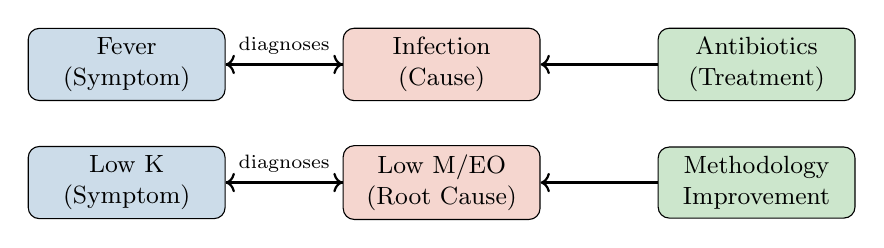
\begin{tikzpicture}[
    box/.style={rectangle, draw, rounded corners, minimum width=2.5cm, minimum height=0.8cm, align=center, font=\small},
    arrow/.style={->, thick}
]

% Medical analogy
\node[box, fill=eslblue!20] (fever) at (0, 1.5) {Fever\\(Symptom)};
\node[box, fill=eslred!20] (infection) at (4, 1.5) {Infection\\(Cause)};
\node[box, fill=eslgreen!20] (treatment) at (8, 1.5) {Antibiotics\\(Treatment)};

\draw[arrow] (infection) -- (fever);
\draw[arrow, dashed] (fever) -- node[above, font=\scriptsize] {diagnoses} (infection);
\draw[arrow] (treatment) -- (infection);

% ESL analogy
\node[box, fill=eslblue!20] (klow) at (0, 0) {Low K\\(Symptom)};
\node[box, fill=eslred!20] (method) at (4, 0) {Low M/EO\\(Root Cause)};
\node[box, fill=eslgreen!20] (intervention) at (8, 0) {Methodology\\Improvement};

\draw[arrow] (method) -- (klow);
\draw[arrow, dashed] (klow) -- node[above, font=\scriptsize] {diagnoses} (method);
\draw[arrow] (intervention) -- (method);

\end{tikzpicture}
\end{center}

\begin{definition}[Diagnostic Function of K]
\label{def:k-diagnostic}
The K-metric serves a \textbf{diagnostic function}: low K-scores indicate the presence of underlying methodological or epistemic problems (low M-Score or EO-Score) that are the true causes of replication failure.

Formally, K is a \textbf{proxy measure} for:
\begin{equation}
K \approx f(M, EO) + \epsilon
\end{equation}
where $f$ captures the systematic relationship between methodology/openness and claim-evidence calibration, and $\epsilon$ represents noise.
\end{definition}

\subsection{Why Does K Work as a Diagnostic?}

The K-metric works as a diagnostic because of systematic co-occurrence:

\begin{enumerate}
    \item \textbf{Poor methodology produces both overclaiming and non-replication.}

    Researchers with weak methods (underpowered studies, no pre-registration, permitted deception) tend to:
    \begin{itemize}
        \item Overclaim because they don't recognize the fragility of their evidence ($\downarrow$ K)
        \item Produce non-replicating findings because their methods are unreliable
    \end{itemize}

    \item \textbf{Strong methodology produces both calibration and replication.}

    Researchers with strong methods (triangulation, pre-registration, no deception) tend to:
    \begin{itemize}
        \item Calibrate claims appropriately because they understand evidence limits ($\uparrow$ K)
        \item Produce replicating findings because their methods are robust
    \end{itemize}
\end{enumerate}

\begin{proposition}[The Diagnostic Mechanism]
\label{prop:diagnostic-mechanism}
Let $M$ denote methodology quality and $R$ denote replication probability. Then:
\begin{equation}
\text{Cov}(K, R) = \text{Cov}(K, M) \cdot \beta_{MR} + \text{Cov}(K, \epsilon_R)
\end{equation}
where $\beta_{MR}$ is the effect of methodology on replication.

Since $\text{Cov}(K, M) > 0$ and $\beta_{MR} > 0$, we have $\text{Cov}(K, R) > 0$ even though $K$ has no causal effect on $R$.
\end{proposition}

\subsection{Implications for K-Metric Interpretation}

\begin{warningbox}[title={ESL 2.3: Revised Interpretation Guidelines}]
\textbf{Old interpretation} (ESL 1.0--2.2):
\begin{itemize}
    \item Low K $\Rightarrow$ ``This claim is poorly calibrated and therefore risky.''
    \item High K $\Rightarrow$ ``This claim is well calibrated and therefore reliable.''
\end{itemize}

\textbf{New interpretation} (ESL 2.3):
\begin{itemize}
    \item Low K $\Rightarrow$ ``This claim shows signs of underlying methodological weakness. Check M-Score and EO-Score.''
    \item High K $\Rightarrow$ ``This claim shows signs of methodological strength, but confirm with M-Score and EO-Score.''
\end{itemize}

The K-metric is a \textbf{screening tool}, not a verdict.
\end{warningbox}

\subsection{The ESL 2.3 Assessment Workflow}

\begin{definition}[ESL 2.3 Full Assessment]
\label{def:full-assessment}
The complete ESL 2.3 assessment includes:

\begin{enumerate}
    \item \textbf{K-Score} (Screening): Compute $K = \min(B, E) / \max(B, E)$
    \item \textbf{M-Score} (Methodology): Assess 7-factor methodology quality (Appendix G)
    \item \textbf{EO-Score} (Openness): Assess 5-factor epistemic openness (Appendix H)
    \item \textbf{Integrated Assessment}:
    \begin{equation}
    \text{Risk} = f(\text{Low } K, \text{Low } M, \text{Low } EO)
    \end{equation}
\end{enumerate}
\end{definition}

\begin{table}[h]
\centering
\caption{ESL 2.3 Integrated Interpretation Matrix}
\label{tab:integrated-matrix}
\begin{tabular}{cccl}
\toprule
\textbf{K} & \textbf{M} & \textbf{EO} & \textbf{Interpretation} \\
\midrule
High & High & High & Highly reliable (expected replication $>$ 90\%) \\
High & High & Low & Reliable but verify openness practices \\
High & Low & High & Unusual---investigate methodology \\
High & Low & Low & False positive K; actual risk is high \\
\midrule
Low & High & High & Linguistic issue only; substance is solid \\
Low & High & Low & Mixed signals; investigate further \\
Low & Low & High & Methodology issue; improve methods \\
Low & Low & Low & High risk (expected replication $<$ 30\%) \\
\bottomrule
\end{tabular}
\end{table}

\begin{keyinsight}[title={The Key Implication}]
\textbf{Treat the infection, not the fever.}

When K is low:
\begin{itemize}
    \item Don't just rewrite the claims (``reducing fever'').
    \item Investigate and improve methodology and epistemic practices (``treating infection'').
    \item K will improve as a natural consequence.
\end{itemize}
\end{keyinsight}

% =============================================================================
% 2.10 COMPUTATIONAL CONSIDERATIONS
% =============================================================================

\section{Computational Considerations}
\label{sec:computation}

\subsection{Algorithm}

\begin{table}[h]
\centering
\caption{K-Metric Computation Algorithm}
\label{tab:algorithm}
\begin{tabular}{ll}
\toprule
\textbf{Step} & \textbf{Operation} \\
\midrule
1 & Input: $B, E \in [0, 1]$ \\
2 & If $B = 0$ and $E = 0$: return $K = 1$ \\
3 & Compute $M = \max(B, E)$ \\
4 & Compute $D = |B - E|$ \\
5 & Return $K = 1 - D / M$ \\
\bottomrule
\end{tabular}
\end{table}

\textbf{Complexity}: $O(1)$ for single claim; $O(n)$ for document with $n$ claims.

\subsection{Numerical Stability}

For very small values of $B$ and $E$ (approaching machine epsilon), use:
\begin{equation}
K = \frac{\min(B, E)}{\max(B, E) + \epsilon}
\end{equation}
where $\epsilon \approx 10^{-10}$ prevents division by zero.

\subsection{Implementation}

\begin{verbatim}
def k_metric(B: float, E: float, eps: float = 1e-10) -> float:
    """Compute the standard K-metric."""
    if B < eps and E < eps:
        return 1.0  # Perfect calibration at null claim
    return min(B, E) / (max(B, E) + eps)

def k_asymmetric(B: float, E: float, alpha: float = 0.5) -> float:
    """Compute asymmetric K-metric (penalizes overclaiming)."""
    if abs(B - E) < 1e-10:
        return 1.0
    if B > E:  # Overclaiming
        return E / B
    else:  # Underclaiming
        return 1 - alpha * (E - B) / E
\end{verbatim}

% =============================================================================
% 2.11 CHAPTER SUMMARY
% =============================================================================

\section{Chapter Summary}
\label{sec:summary}

This chapter has established the mathematical foundations of the K-metric and its role in ESL 2.3:

\begin{enumerate}
    \item \textbf{Axiomatic Foundation}: Five required axioms (boundedness, perfect calibration, monotonicity, continuity, non-triviality) and two optional axioms (symmetry, zero at maximum deviation) constrain the space of valid calibration metrics.

    \item \textbf{Standard K-Metric}: $K = 1 - |B - E| / \max(B, E) = \min(B, E) / \max(B, E)$ satisfies all axioms and provides a symmetric, scale-invariant measure of calibration.

    \item \textbf{Asymmetric Variant}: $K_{\text{asym}}$ penalizes overclaiming more severely than underclaiming, appropriate for conservative scientific communication.

    \item \textbf{Geometric Interpretation}: K-values correspond to rays from the origin in B-E space; the calibration line ($B = E$) represents $K = 1$.

    \item \textbf{Algebraic Properties}: The K-metric is scale-invariant, has clean partial derivatives, and connects to logarithmic distance measures.

    \item \textbf{Aggregation Rules}: Weakest-Link Aggregation (WLA) for dependent claims; arithmetic or weighted mean for independent claims.

    \item \textbf{Error Propagation}: First-order formulas enable uncertainty quantification when $B$ and $E$ are measured with error.

    \item \textbf{Related Metrics}: K connects to Brier score, Expected Calibration Error, and KL divergence while providing a simpler, bounded alternative.

    \item \textbf{Diagnostic Interpretation (ESL 2.3)}: The K-metric functions as a \textbf{diagnostic indicator}, not a causal predictor. B-value shows $r = 0.052$ with replication; the true predictors are M-Score ($r = 0.901$) and EO-Score ($r = 0.954$). Low K signals underlying methodological weakness---``treat the infection, not the fever.''

    \item \textbf{Integrated Assessment}: ESL 2.3 combines K-screening with M-Score and EO-Score assessment for comprehensive quality evaluation.
\end{enumerate}

\begin{eslbox}
\textbf{Chapter 2 Self-Assessment (ESL 2.3)}

This chapter presents mathematical definitions and proofs ($B \approx 0.85$) derived through formal reasoning, plus empirical findings from N=119 validation ($E \approx 0.90$).

\textbf{Calculation}: $K = 1 - |0.85 - 0.90| / 0.90 = 1 - 0.056 = 0.94$

\textbf{Status}: \textcolor{eslgreen}{\textbf{Highly Stable}} ($K \geq 0.90$)

\textbf{Claim Types}:
\begin{itemize}
    \item Axioms and definitions: T3 (Mathematical construction)
    \item Theorems and proofs: T3 (Formal derivation)
    \item Relationship to other metrics: T2 (References established literature)
    \item Diagnostic interpretation: T1 (Empirically validated, N=119)
    \item Predictor correlations: T1 (Empirical data)
    \item Recommended defaults (e.g., $\alpha = 0.5$): T4 (Expert proposal)
\end{itemize}

\textbf{Diagnostic Check}: This chapter's high K-score is consistent with strong M-Score (formal mathematical methodology) and high EO-Score (transparent derivations, connection to established literature).
\end{eslbox}

% =============================================================================
% REFERENCES
% =============================================================================

\newpage
\bibliographystyle{apalike}

\begin{thebibliography}{99}

\bibitem[Brier, 1950]{Brier1950}
Brier, G. W. (1950).
Verification of forecasts expressed in terms of probability.
\textit{Monthly Weather Review}, 78(1), 1--3.

\bibitem[Gneiting \& Raftery, 2007]{Gneiting2007}
Gneiting, T., \& Raftery, A. E. (2007).
Strictly proper scoring rules, prediction, and estimation.
\textit{Journal of the American Statistical Association}, 102(477), 359--378.

\bibitem[Kullback \& Leibler, 1951]{Kullback1951}
Kullback, S., \& Leibler, R. A. (1951).
On information and sufficiency.
\textit{The Annals of Mathematical Statistics}, 22(1), 79--86.

\bibitem[Naeini et al., 2015]{Naeini2015}
Naeini, M. P., Cooper, G., \& Hauskrecht, M. (2015).
Obtaining well calibrated probabilities using Bayesian binning.
\textit{Proceedings of the AAAI Conference on Artificial Intelligence}, 29(1).

\end{thebibliography}

\end{document}
